\section{Transformer-XL} \label{sec:TransformerXL}

\subsection{Problem With Transformer: Context-Fragmentation Problem} \label{sec:ContextFragmentationProblem}


\begin{figure}[h]
\vspace{-5pt}
\centering
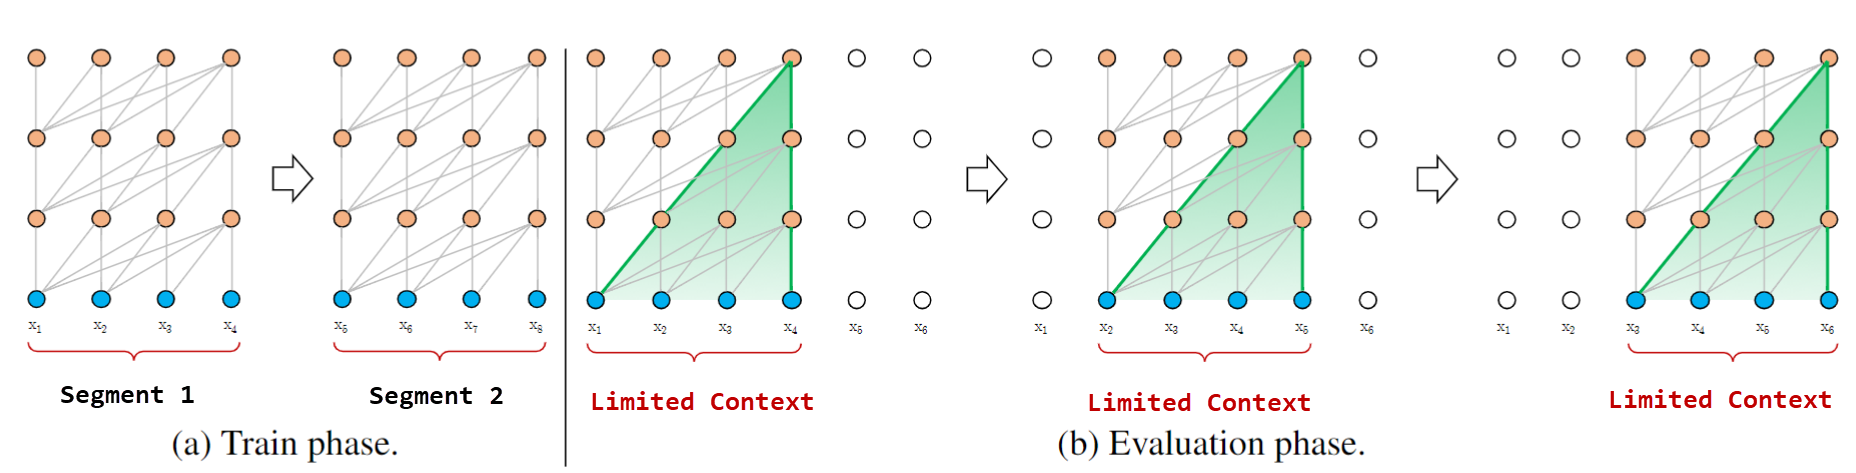
\includegraphics[width=\linewidth]{imgs/transXL_vanillaSegmentation.png}
%\vspace{-5pt}
\caption{Vanilla \nameref{sec:Transformer} with segment embedding length $ = 4$. During each evaluation step, the \nameref{sec:Transformer} consumes a segment embedding and makes a prediction at the last position. Next, the segment is shifted one position, so the new segment must be processed from scratch, \hyperref[sec:ContextFragmentationProblem]{breaking context dependency} between first tokens of each segment and between segments. From \emph{Transformer-XL: Attentive Language Models Beyond a Fixed-Length Context}, by Dai et al., 2019. \url{https://arxiv.org/pdf/1901.02860.pdf}. Copyright 2019 by Dai et al.}
%\vspace{-5pt}
\label{fig:transXL_VanillaSegment}
\end{figure}

\nameref{sec:Transformer}s cannot learn long-term dependencies because of {\label{sec:FixedLengthContext} \textbf{fixed-length context}}, or context that is limited by input length (Dai et al., 2019). The \emph{vanilla} (ordinary) \nameref{sec:Transformer} model adapted by Al-Rfou et al. (2018) uses fixed-length context since the model is trained within its segment embeddings, blocking information from flowing across segment embeddings during forward and backward propagation passes. %\hyperref[sec:ForwardProp]{forward} and \hyperref[sec:BackwardProp]{backward passes}. 
This result, visible in \cref{fig:transXL_VanillaSegment}, causes the \nameref{sec:Transformer} to forget context from previous segments. This is termed the \textbf{context fragmentation problem}.


\subsection{Motivation for Transformer-XL} \label{sec:MotivationForTransformerXL}

\textbf{Transformer-XL} (extra long) avoids ``disrupting temporal coherence." Instead of breaking up sequences into arbitrary \textbf{fixed lengths}, the Transformer-XL \emph{respects natural language boundaries} like sentences and paragraphs, helping it gain richer context over these and longer texts like documents. Through the use of \hyperref[sec:SegmentLevelRec]{segment-level recurrence mechanism} and \hyperref[sec:RelativePosEnc]{relative positional encoding}s, the Transformer-XL can overcome the \hyperref[sec:ContextFragmentationProblem]{context-fragmentation problem} and represent longer-spanning dependencies (Dai et al., 2019). 


\subsection{Describing Transformer-XL} \label{sec:DescribingTransformerXL}

\subsubsection{Segment-Level Recurrence Mechanism} \label{sec:SegmentLevelRec}

To resolve the \hyperref[sec:ContextFragmentationProblem]{context fragmentation problem}, the Transformer-XL employs a \textbf{segment-level recurrence mechanism} to capture long-term dependencies using information from previous segments. When a segment is being processed, each hidden layer receives two inputs: ($1$) the previous hidden layer outputs of the \emph{current segment} (akin to the vanilla model, shown as gray arrows in \cref{fig:transXL_extendedContext}), and ($2$) the previous hidden layer outputs of the \emph{previous segment} (green arrows in \cref{fig:transXL_extendedContext}). So although gradient updates or training still occurs within a segment, this extended context feature lets historical information to be fully used, avoiding \hyperref[sec:ContextFragmentationProblem]{context fragmentation}. 


\begin{figure}[h]
%\vspace{-5pt}
\centering
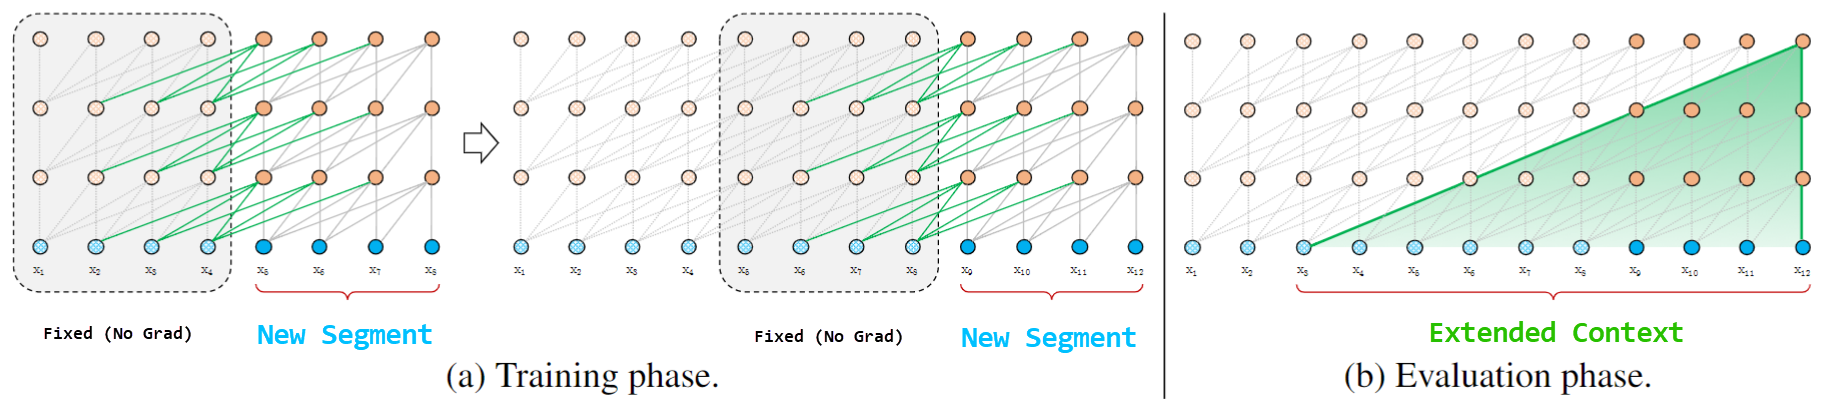
\includegraphics[width=\linewidth]{imgs/transXL_extendedcontext.png}
%\vspace{-5pt}
\caption{Segment level recurrence mechanism at work: the hidden state for previous segment is \emph{fixed} and \emph{stored} to later be reused as an extended context while the new segment is processed. Like in \nameref{sec:Transformer}, gradient updates or training still occurs within a segment, but the extended context feature allows historical information to now be incorporated. From \emph{Transformer-XL: Attentive Language Models Beyond a Fixed-Length Context}, by Dai et al., 2019. \url{https://arxiv.org/pdf/1901.02860.pdf}. Copyright 2019 by Dai et al.}
%\vspace{-20pt}
\label{fig:transXL_extendedContext}
\end{figure}


Intuitively, for the sentence ``I went to the store. I bought some cookies," the model receives the sentence ``I went to the store," caches the hidden states, and only \emph{then} feeds the remaining sentence ``I bought some cookies" and cached hidden states together into the model (Kurita, 2019b). 

To formally describe the recurrence mechanism, let $\textbf{s}_\tau = \Big\{ x_{\tau_1}, x_{\tau_2}, ..., x_{\tau_L} \Big\}$ and $\textbf{s}_{\tau + 1} = \Big\{ x_{{\tau+1}_1}, x_{{\tau+1}_2}, ..., x_{{\tau+1}_L} \Big\}$ denote two consecutive segment embeddings of length $L$. Let $\textbf{h}_\tau^n \in \mathbb{R}^{L \times d}$ be the $n$-th layer's hidden state vector produced for the $\tau$-th segment $\textbf{s}_\tau$, where $d$ is the hidden dimension. Then $n$-th layer's hidden state for next segment $\textbf{s}_{\tau + 1}$ is calculated in \cref{eq:TransXLHiddens} as:


\begin{equation}
\begin{array}{ll}
\Tilde{\textbf{h}}_{\tau + 1}^{n-1} = \Big\{ \texttt{StopGradient}\Big( \textbf{h}_\tau^{n-1} \circ \textbf{h}_{\tau+1}^{n-1} \Big) \Big\} \\\\
%
\textbf{q}_{\tau+1}^n, \;\;\; \textbf{k}_{\tau+1}^n, \;\;\; \textbf{v}_{\tau+1}^n = \textbf{h}_{\tau+1}^{n-1} \cdot \textbf{W}_q^T, \;\;\; \Tilde{\textbf{h}}_{\tau+1}^{n-1} \cdot \textbf{W}_k^T, \;\;\; \Tilde{\textbf{h}}_{\tau+1}^{n-1} \cdot \textbf{W}_v^T \\\\
%
\textbf{h}_{\tau+1}^n = \texttt{TransformerLayer} \Big( \textbf{q}_{\tau+1}^n, \;\;\; \textbf{k}_{\tau+1}^n \;\;\; \textbf{v}_{\tau+1}^n \Big)
\end{array}
\label{eq:TransXLHiddens}
\end{equation}



where the first line indicates that the two consecutive hidden states are concatenated; $\textbf{W}$ denotes model parameters; and $\textbf{q}, \textbf{k}, \textbf{v}$ are the \hyperref[sec:QKV]{query, key, and value vectors}. The key feature here, compared to standard \nameref{sec:Transformer}, is that the key $\textbf{k}_{\tau+1}^n$ and value $\textbf{v}_{\tau+1}^n$ are conditioned on the elongated context $\Tilde{\textbf{h}}_{\tau+1}^{n-1}$ \emph{and} the previous segment's cached context $\textbf{h}_\tau^{n-1}$. This is visible by the green lines in \cref{fig:transXL_extendedContext}.  

This new recurrence scheme allows more efficient computations. Also, it can cache multiple previous segments not just the previous one, making it more similar to an \hyperref[sec:RNN]{RNN's memory}. 




\subsubsection{Relative Positional Encoding} \label{sec:RelativePosEnc}

Trying to graft the \nameref{sec:Transformer}'s \hyperref[sec:PosEncodings]{positional encodings} directly with the \hyperref[sec:SegmentLevelRec]{segment-level recurrence mechanism} caused problems. Simply put, the Transformer-XL could not keep positional word order straight when reusing hidden states because tokens from different segments ended up with the same \hyperref[sec:PosEncodings]{positional encodings}, even though their position and importance could differ. This confused the model. 

To remedy this and correctly merge the recurrence scheme with positional word order, the authors invented \textbf{relative \hyperref[sec:PosEncodings]{positional encodings}} that work conjunction with \hyperref[sec:AttentionMechanism]{attention score}s of each layer, as opposed to only before the first layer, and which are based on \emph{relative} not \emph{absolute} distances between tokens (Horev, 2019). Formally speaking, the authors created a relative \hyperref[sec:PosEncodings]{positional encoding}s matrix whose $i$-th row indicates a relative distance of $i$ between two positions, and injected this into the attention module. As a result, the query vector can distinguish between two tokens using their different distances. Now, from Dai et al. and Horev (2019), the attention head calculation has four parts: 

\begin{enumerateSpaced}{3pt}
    \item \textbf{Content-based addressing: }the original attention score without \hyperref[sec:PosEncodings]{positional encoding}.
    
    \item \textbf{Content-dependent positional bias: }with respect to the current query. It uses a sinusoidal function that gets distance between tokens instead of \emph{absolute} position of a current token. 
    
    \item \textbf{Learned global content bias: } is a learned vector that accounts for the other tokens in the key matrix.
    
    \item \textbf{Learned global positional bias: }is a learned vector that adjusts the importance based only on distance between tokens, using the intuition that recent previous words are more relevant that a word from the previous paragraph. 
\end{enumerateSpaced}




\subsection{Experimental Results: Ablation Study for Segment-Level Recurrence and Relative Positional Encodings} \label{sec:ExpResultsTransXL}


% NOTE: secret to make text not overlap is either: 
% (1) enlarging the image just right
% (2) including all possible text after wrapfigure, not including few texts (as much text as possible within the parantheses).

{
\begin{wrapfigure}{L}{0.75\textwidth}
\begin{center}
    \vspace{-20pt}
    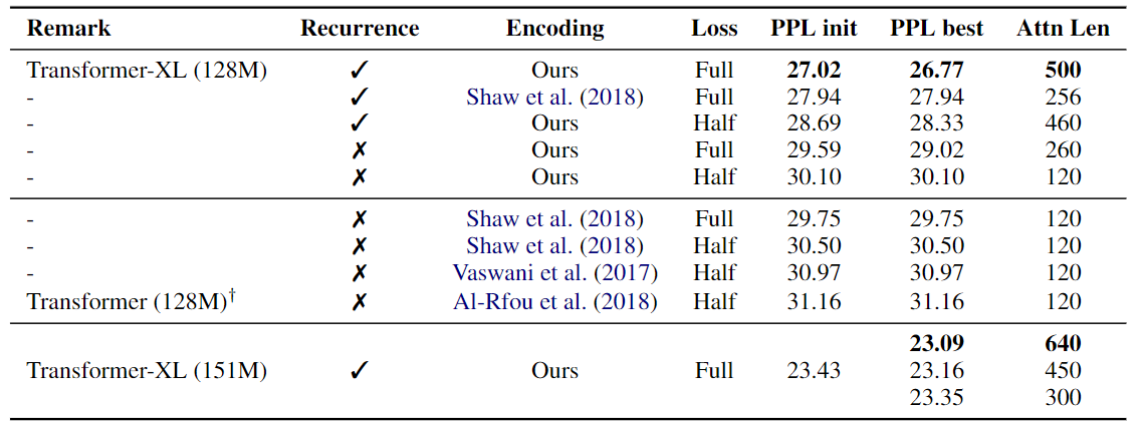
\includegraphics[width=\linewidth]{imgs/table_transXL_ablationREC.png}
\end{center}
\vspace{-20pt}
\captionof{table}{\scriptsize Ablation study for \nameref{sec:SegmentLevelRec} on the WikiText-103 data set. \textbf{PPL best} (model output) means perplexity score obtained using an optimal backpropagation %\hyperref[sec:BackwardProp]{backpropagation} 
training time length. \textbf{Attn Len} (model input) is the shortest possible attention length during evaluation to achieve the corresponding PPL best. From \emph{Transformer-XL: Attentive Language Models Beyond a Fixed-Length Context}, by Dai et al., 2019. \url{https://arxiv.org/pdf/1901.02860.pdf}. Copyright 2019 by Dai et al.}
\vspace{25pt}
\label{tbl:transXL_ablationRECURR}
\end{wrapfigure}

The authors seek to isolate the effects of Transformer-XL's \hyperref[sec:SegmentLevelRec]{segment-level recurrence mechanism} using with different encoding schemes. In \cref{tbl:transXL_ablationRECURR}, Shaw et al. (2018) uses relative encodings, and Vaswani and Al-Rfou use absolute encodings. 

In \cref{tbl:transXL_ablationRECURR}, \hyperref[sec:SegmentLevelRec]{segment-level recurrence} and \hyperref[sec:RelativePosEnc]{relative positional encoding} must be used in conjunction for best performance, since when using the new recurrence with the new encodings, the Transformer-XL can generalize to larger attention sequences (with length $500$) during evaluation while getting lowest perplexity score of $26.7$. 


However, if the Transformer-XL just uses the new encodings, even using shorter attention sequences of $260$ and $120$ with different backprop loss schemes cannot help lower its perplexity scores, as shown in the last two rows of \cref{tbl:transXL_ablationRECURR}'s Transformer-XL section. The standard \nameref{sec:Transformer} does poorly in general, showing high overall perplexities even using short attention lengths. 
}